
\documentclass[crop,tikz]{standalone}
\usepackage[utf8]{inputenc}
\usepackage{tikz}
\usepackage{pgfplots}
\pgfplotsset{compat=newest}
\usepgfplotslibrary{groupplots}
\begin{document}
% This file was created by matplotlib2tikz v0.6.18.
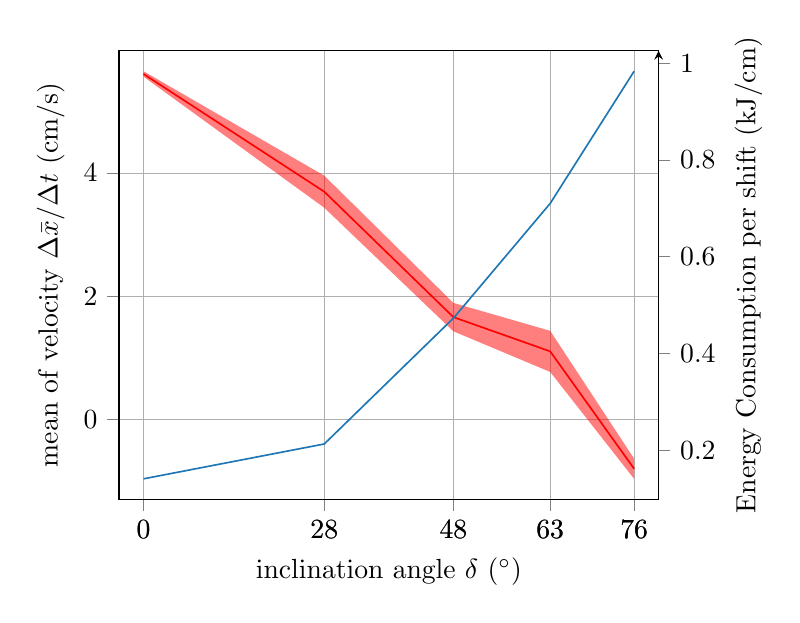
\begin{tikzpicture}

\definecolor{color0}{rgb}{0.12156862745098,0.466666666666667,0.705882352941177}

\begin{axis}[
tick align=outside,
tick pos=left,
x grid style={lightgray!92.02614379084967!black},
xlabel={inclination angle $\delta$ ($^\circ$)},
xmajorgrids,
xmin=-3.8, xmax=79.8,
xtick={0, 28, 48, 63, 76},
y grid style={lightgray!92.02614379084967!black},
ylabel={mean of velocity $\Delta \bar{x} / \Delta t$ (cm/s)},
ymajorgrids,
ymin=-1.29364531282406, ymax=5.98374757284272
]
\path [fill=red, fill opacity=0.5] (axis cs:0,5.56499991062033)
--(axis cs:0,5.65295698713059)
--(axis cs:28,3.95820563639983)
--(axis cs:48,1.89297743831517)
--(axis cs:63,1.43933570167321)
--(axis cs:76,-0.635998283251234)
--(axis cs:76,-0.96285472711193)
--(axis cs:76,-0.96285472711193)
--(axis cs:63,0.772051846422663)
--(axis cs:48,1.43146918808684)
--(axis cs:28,3.43746525645888)
--(axis cs:0,5.56499991062033)
--cycle;

\addplot [semithick, red, forget plot]
table [row sep=\\]{%
0	5.60897844887546 \\
28	3.69783544642935 \\
48	1.66222331320101 \\
63	1.10569377404794 \\
76	-0.799426505181582 \\
};
\end{axis}

\begin{axis}[
axis y line=right,
tick align=outside,
x grid style={lightgray!92.02614379084967!black},
xmin=-3.8, xmax=79.8,
xtick pos=left,
xtick={0, 28, 48, 63, 76},
y grid style={lightgray!92.02614379084967!black},
ylabel={Energy Consumption per shift (kJ/cm)},
ymin=0.0988321939217474, ymax=1.0253921467144,
ytick pos=right
]
\addplot [semithick, color0, forget plot]
table [row sep=\\]{%
0	0.140948555412323 \\
28	0.212947862405971 \\
48	0.472822679347774 \\
63	0.710105096894192 \\
76	0.983275785223828 \\
};
\end{axis}

\end{tikzpicture}
%% End matplotlib2tikz content %% 
\end{document}